\section{ETL/ELT процессы. Хранилища, витрины, озёра данных.}

\D{
    ETL - extract trasnform load. Получаем данные, приводим их
    к стандартному виду для загрузки в хранилище, а затем постоянно
    достаем из хранилища.
}

\D{
    ELT - получение данных с минимальной трансформацией. Помещение их в
    хранилище для последующего доступа и дальнейшей трансформации.
}

\begin{figure}[H]
	\centering
	\begin{minipage}[b]{0.6\textwidth}
		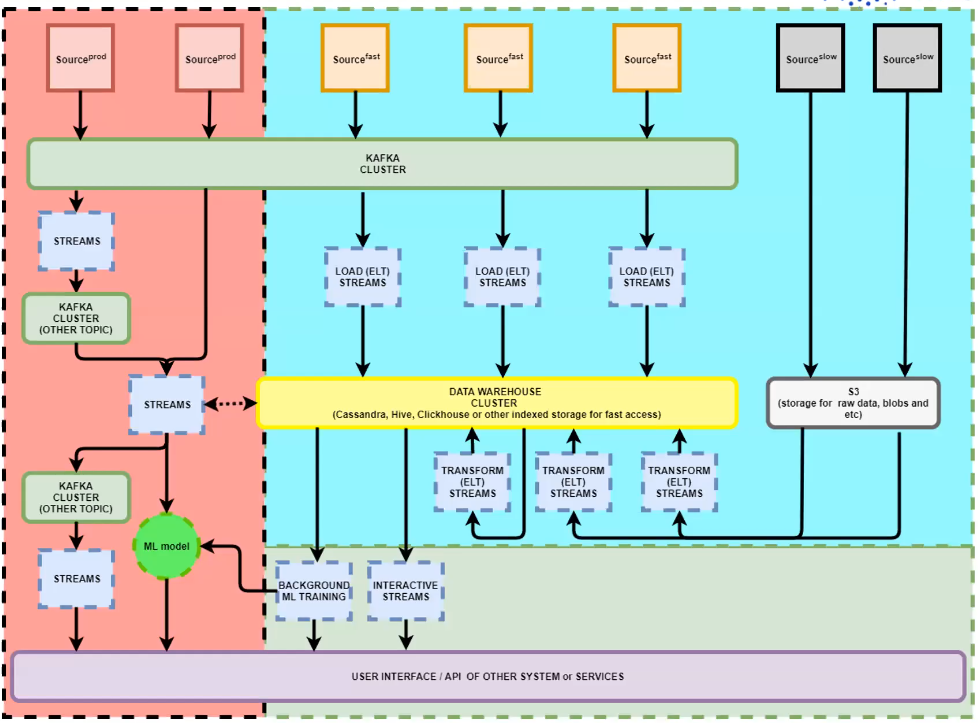
\includegraphics[width=\textwidth]{images/etl.png}
		\caption{ETL process}
	\end{minipage}
\end{figure}